\documentclass{beamer}
\usetheme{Warsaw}
\useinnertheme{circles}
\useoutertheme[subsection=false]{smoothbars}
\usepackage[utf8x]{inputenc}
\usepackage[czech]{babel}
\usepackage[T1]{fontenc}
\usepackage{listings}
\usepackage{tikz}
\lstset{basicstyle=\tiny\ttfamily}
\logo{
\includegraphics[height=0.5cm]{brmlab.pdf}}

\begin{document}

\AtBeginSection[]
{
  \begin{frame}
    \frametitle{Outline}
    \tableofcontents[currentsection]
  \end{frame}
}

\title{brmiversity: Umělá inteligence \\ a teoretická informatika}
\subtitle{Přednáška č. 7}
\author{Petr Baudiš $\langle${\tt pasky@ucw.cz}$\rangle$}
\institute{
	brmlab 2011\\
	\vskip 1ex
	\pgfdeclareimage[height=4ex]{ccbysa}{by-sa.pdf}
	\pgfuseimage{ccbysa}
}
\date{}
\frame{\titlepage}

\section{Umělá inteligence}

\subsection{}
\begin{frame}{Zpracování neurčité informace}
\begin{itemize}
\item Data o světě jsou neurčitá
\item Úkony ve světě jsou neurčité
\item \dots takže reálný svět je neurčitý
\item Minule jsme modelovali arbitrární vztahy mezi jevy
\item Dnes budeme modelovat {\em procesy} a {\em vstupy}
\end{itemize}
\end{frame}

\subsection{}
\begin{frame}{Markovovský řetězec}
\begin{itemize}
\item Posloupnost stavů splňujících {\em Markovovu vlastnost}
\item Každý stav závisí (stochasticky) pouze na předchozím; {\bf nemáme paměť}
\item $k$-tého řádu: Závislost na $k$ předchozích
\item (Je to ekvivalentní?)
\vskip 3ex
\pause
\item Velmi zjednodušený model, ale výpočetně triviální a dobrá aproximace
\item Množina stavů, pravděpodobnosti přechodu mezi stavy
\end{itemize}

TODO ilustrace
\end{frame}

\subsection{}
\begin{frame}{Muaddib}
\begin{center}
{\tt
<TomSuch> 1+1 \\
<Muaddib> Kde jsou vsichni mimo kretena 1... \\ Senat souhlasi... Poslanecka snemovna nesouhlasi... Kreteni jsou vsichni.
}
\end{center}

\vskip 3ex
\pause

TODO: Puvodni vety z logu.

\vskip 3ex
\pause

\begin{itemize}
\item Symboly (stavy) pro slova a neslova (okraj věty: Slovo $\epsilon$)
\item Dva MM 4. řádu --- 3 slova před, 3 slova po
\item Vstup: Update MM, pevné body, doplnění věty z MM
\end{itemize}
\end{frame}

\subsection{}
\begin{frame}{Skrytý Markovovský řetězec (HMM)}
TODO ilustrace

\begin{itemize}
\item {\em Skryté} stavy nedokážeme pozorovat, viditelné projevy jsou asociovány pouze stochasticky
\item Pravděpodobnost přechodu mezi stavy {\em a} pravděpodobnost jevu $X$ ve stavu $A$
\item (Pomocí Bayesovského pravidla můžeme podle jevu určit pravděpodobnost různých stavů)
\item Učení: TODO
\end{itemize}
\vskip 3ex
\pause
\begin{block}{Inference}
\begin{itemize}
\item Vysvětlování --- jaké stavy jsme prošli?
\item Filtrování --- v jakém stavu právě jsme?
\item Vyhlazování --- v jakém stavu jsme byli tuhle?
\item Pravděpodobnost pozorování
\end{itemize}
\end{block}
\end{frame}

\subsection{}
\begin{frame}{Algoritmy pro HMM}
\begin{block}{Forward algoritmus}
\begin{itemize}
\item TODO
\end{itemize}
\end{block}
\begin{block}{Viterbiho algoritmus}
\begin{itemize}
\item TODO
\end{itemize}
\end{block}
\end{frame}

\subsection{}
\begin{frame}{Opakování: Normální rozdělení}
\begin{columns}
	\begin{column}{5.5cm}
		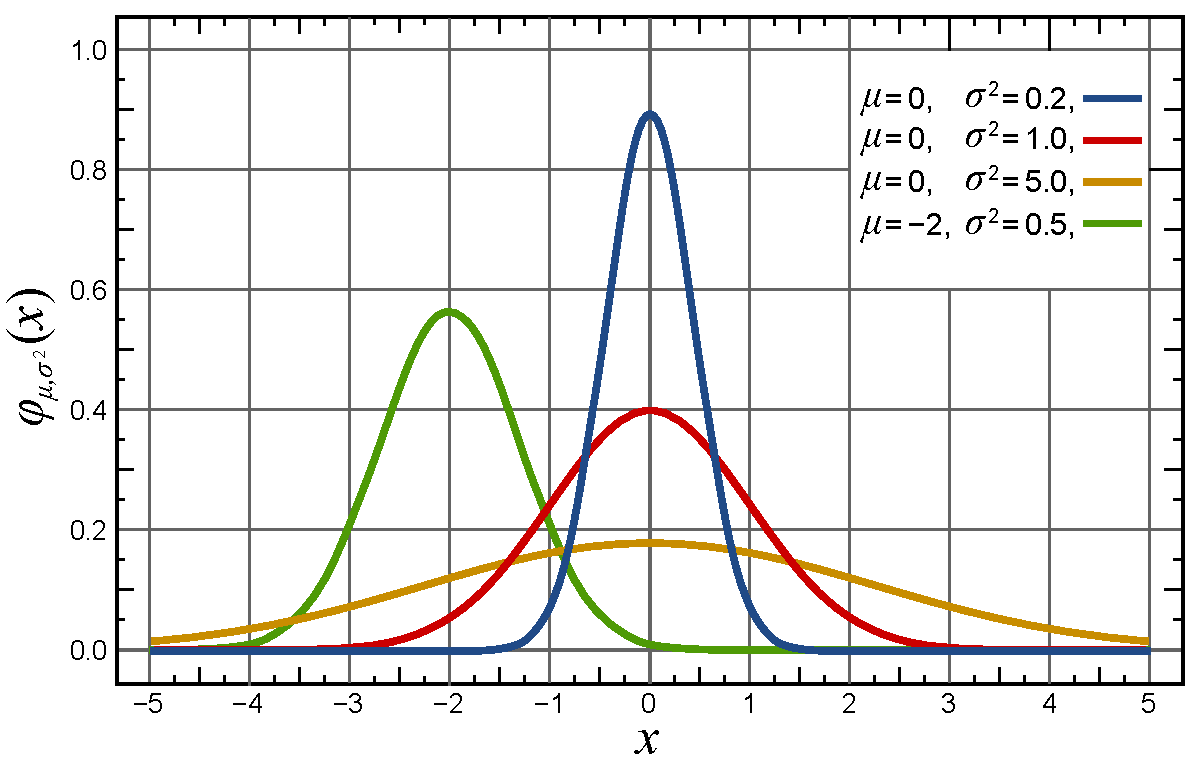
\includegraphics[width=5.5cm]{Normal_Distribution_PDF.pdf}
	\end{column}
	\begin{column}{5.5cm}
		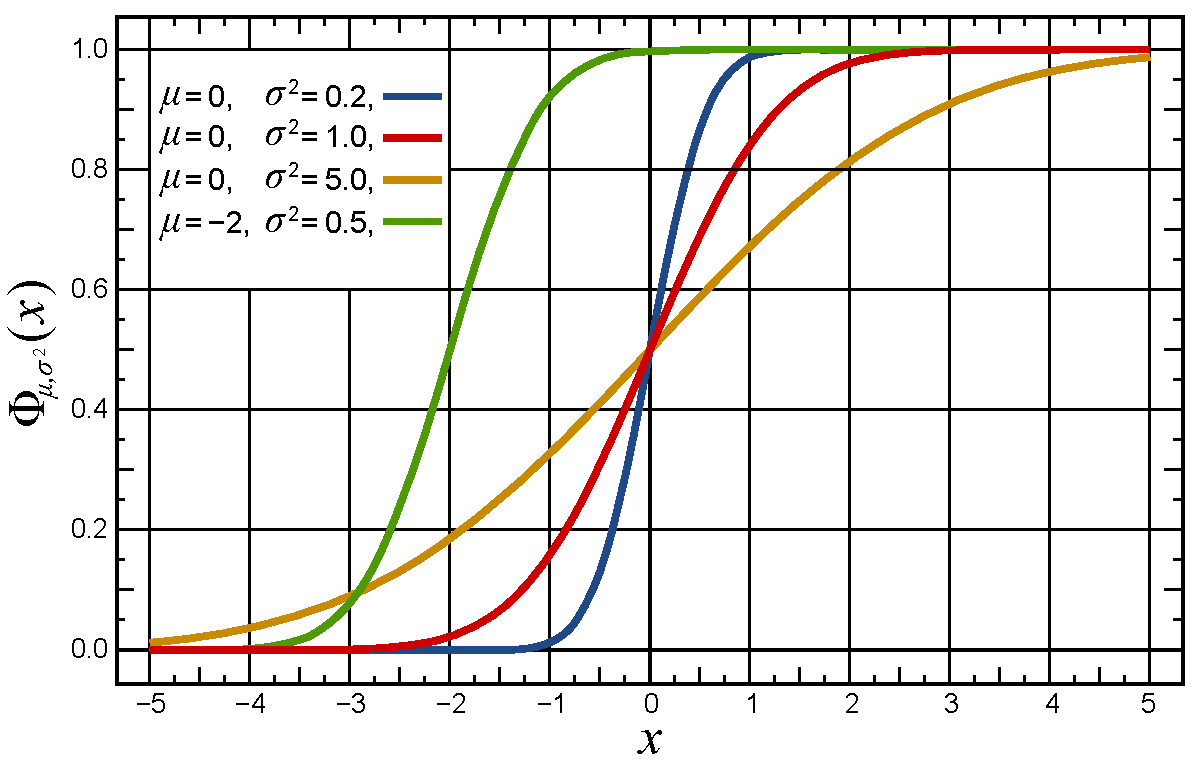
\includegraphics[width=5.5cm]{Normal_Distribution_CDF.pdf}
	\end{column}
\end{columns}

\begin{center}
{\bf Interval spolehlivosti:} S pravděpodob. $p$ bude $\mathbb{E}[X] = \mu \pm \epsilon$

{\em ``LHC detekovalo 130 GeV signaturu na tři sigma.''}
\end{center}
\end{frame}

\subsection{}
\begin{frame}{Kálmánovy filtry}
\begin{itemize}
\item {\bf Lineární dynamický systém} --- HMM se ``spojitými stavy'' a stavy i pozorováními normálně rozdělenými
\item Aneb: Pozorování jsou čísla dle stavů, ale zašuměná dle normálního rozdělení
\item Různá čísla indikují (s omezenou pravděpodobností) různé stavy
\end{itemize}
\end{frame}

\subsection{}
\begin{frame}{Otázky?}
\begin{center}
Příště: Strojové učení (rozhodovací stromy, \\ Bayesovský klasifikátor\dots)
\end{center}
\end{frame}

\section{Neuronové sítě}

\subsection{}
\begin{frame}{Data}
\begin{itemize}
\item Kovariance: Jevy $X$ a $Y$ na sobě nějak závisejí ($\mathbb{E}X\mathbb{E}Y - \mathbb{E}(XY)$)
\item Korelace: Míra závislosti (rozptylová korekce)
\item Jsou-li data v NN korelovaná, jsou redundantní a nesou špatně rozlišitelné informace
\item Jak složitá data chci vlastně umět rozpoznávat?
\end{itemize}
\begin{columns}
\begin{column}{5.5cm}
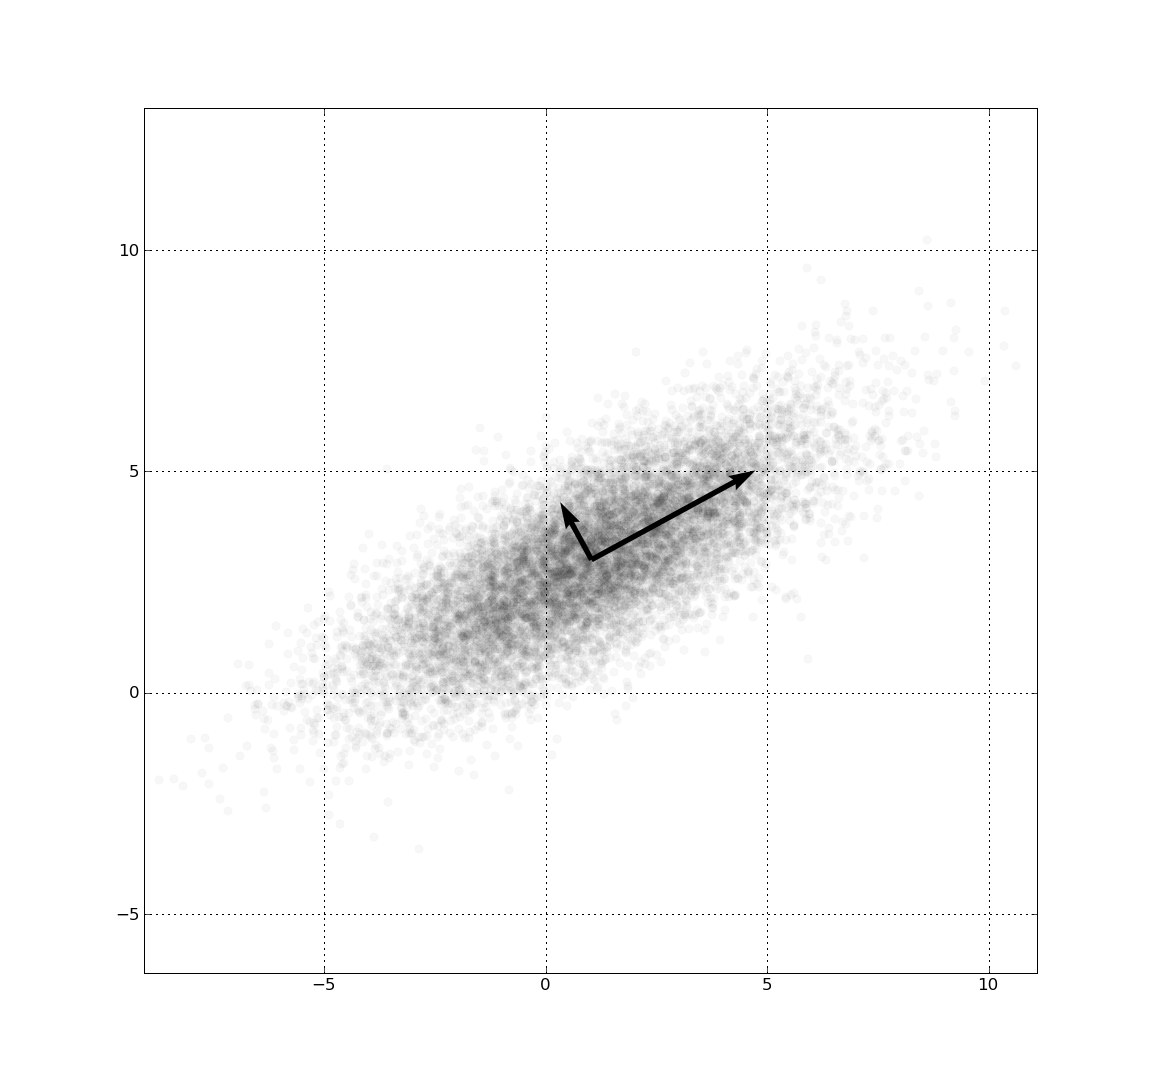
\includegraphics[width=5cm]{GaussianScatterPCA.png}
\end{column}
\begin{column}{5.5cm}
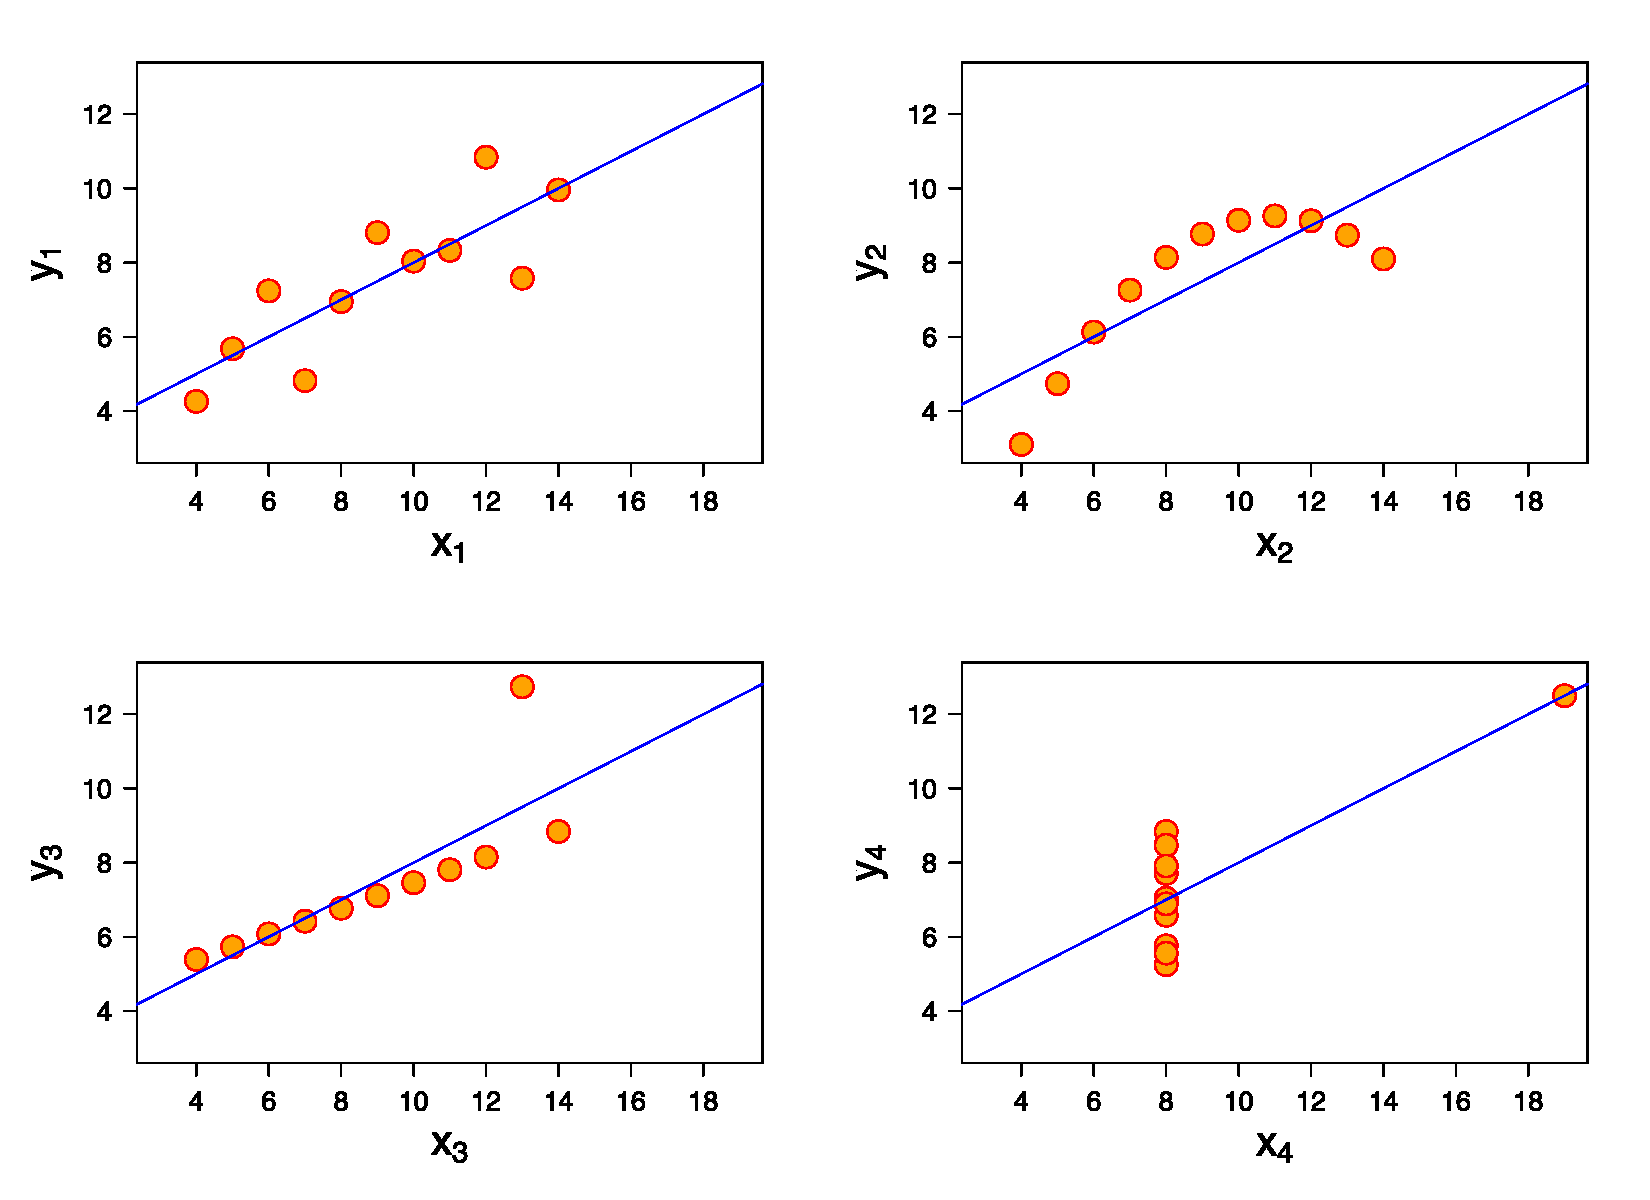
\includegraphics[width=5.5cm]{Anscombe's_quartet_3.pdf}
\end{column}
\end{columns}
\end{frame}

\subsection{}
\begin{frame}{Vapnik-Chervonenkisova dimenze}
\begin{itemize}
\item VC dimenze udává ``kapacitu'' klasifikátoru
\item Nejmenší počet bodů, které lze rozložit do konfigurace, kterou nedokáže klasifikátor rozbít
\item Např. lineární klasifikátor (perceptron) má dimenzi 3
\end{itemize}
\begin{center}
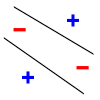
\includegraphics[height=3cm]{VC4.png}
\end{center}
\end{frame}

\subsection{}
\begin{frame}{Principial Component Analysis}
\begin{itemize}
\item Chceme dekolerovat sadu proměnných (dimenze)
\item PCA rozebere oblak dat na jeho ``osy''
\item Dataset $X$ $\to$ dataset $Y$ nižší dimenze
\item Alternativa: Ojův algoritmus
\end{itemize}

\begin{columns}
\begin{column}{6cm}
\begin{block}{Algoritmus}
\begin{itemize}
\item Normalizace podle $\mathbb{E}X$ a $\sigma_E$
\item Kovarianční (disperzní) matice $C$
\item Vybereme vlastní vektory $C$ s nejvyšší energií ($D$)
\item Vstupní vektory projektujeme do vekt. prostoru s bází $D$
\end{itemize}
\end{block}
\end{column}
\begin{column}{5cm}
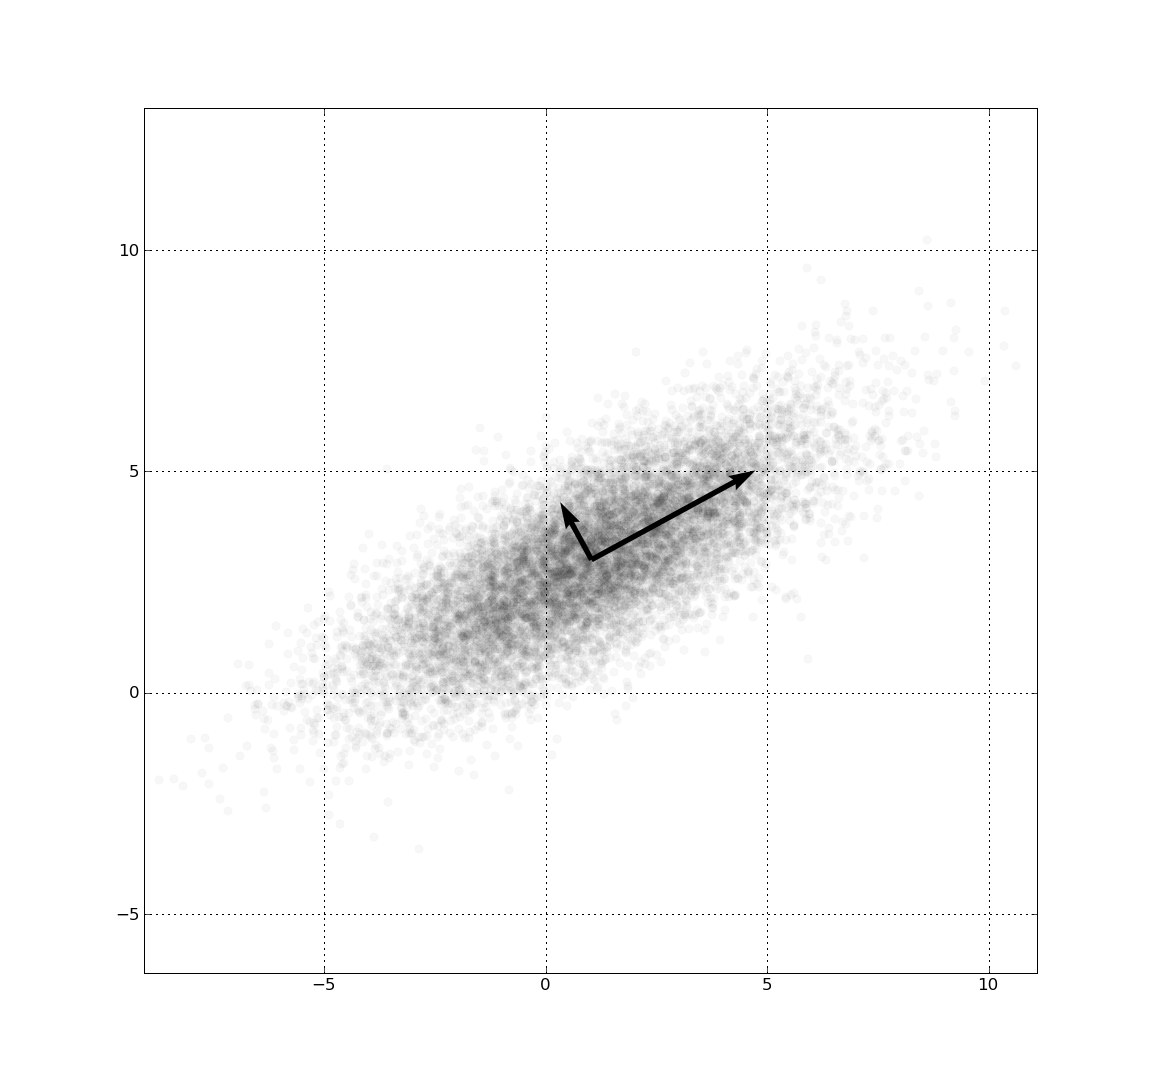
\includegraphics[width=5cm]{GaussianScatterPCA.png}
\end{column}
\end{columns}
\end{frame}

\subsection{}
\begin{frame}{Otázky?}
\begin{center}
Příště: Vylepšení backpropagation, struktura neuronových sítí.
\end{center}
\end{frame}

\section{Adaptivní agenti}

\subsection{}
\begin{frame}{Víceagentní systémy}
\begin{itemize}
\item Peer2peer systém
\item Agenti mohou vznikat, zanikat, potkávat se, pohybovat se
\item Agenti mohou něco chtít od ostatních nebo nabídnout ostatním
\item Ontologie: Soubor znalostí o světě (sada axiomů)
\vskip 3ex
\pause
\item Emergentní chování (``implicitní'' komunikace) \\ vs. pravidla a protokoly
\item Znalosti v multiagentních systémech
\end{itemize}
\end{frame}

\subsection{}
\begin{frame}{Znalosti v multiagentních systémech}
\begin{itemize}
\item Agenti mají znalosti, některé vědí všichni, některé jen skupina, některé jen jeden
\item Pohádka o zablácených dětech
\item Kripkeho sémantika možných světů: Multiverse prořezané znalostmi agenta
\item Modální logika: Logika s predikáty $K_i p$ (agent $i$ ví $p$);
	formalismus (čtvereček a diamant) a spousta vět
\end{itemize}
\end{frame}

\subsection{}
\begin{frame}{Složitější problémy distribuovaných systémů}
\begin{itemize}
\item Byzantští generálové
\item Synchronizace času
\item Ověřování událostí
\end{itemize}
\end{frame}

\subsection{}
\begin{frame}[fragile]{Komunikace v multiagentních systémech}
\begin{itemize}
\item Obvykle externí správce světa (``white page'') nebo nástěnkáři (``yellow page'')
\item FIPA: Foundation for Intelligent Physical Agents
\item Vrstvy: Fyzická, transportní, komunikační, jazyk pro komunikaci agentů (FIPA-ACL, KQML), zprávy (FIPA-SL, Prolog, \dots)
\end{itemize}
\begin{columns}
\begin{column}{4cm}
Změny světa pomocí komunikace, výměna znalostí
\end{column}
\begin{column}[fragile]{7cm}
\begin{lstlisting}
(cfp
 :sender (agent-identifier :name j)
 :receiver (set (agent-identifier :name i))
 :content
  "((action (agent-identifier :name i)
    (sell plum 50))
   (any ?x (and (= (price plum) ?x) (< ?x 10))))"
 :ontology fruit-market
 :language fipa-sl)
\end{lstlisting}
\end{column}
\end{columns}
\end{frame}

\subsection{}
\begin{frame}{Otázky?}
\begin{center}
Příště: Metody pro řízení agentů.
\end{center}
\end{frame}

\section{Datové struktury}

\subsection{}
\begin{frame}{Hashování}
\begin{itemize}
\item Hashovací funkce indexuje hashovací tabulku, řešíme kolize
\item Proč řešíme kolize? Vkládání a mazání (read-write struktura)
\item Perfektní a univerzální hashování
\end{itemize}
\end{frame}

\subsection{}
\begin{frame}{Perfektní hashování}
\begin{itemize}
\item Všechny klíče známe předem, vyrábíme {\em perfektní} hashovací funkci
\end{itemize}
\end{frame}

\subsection{}
\begin{frame}{Univerzální hashování}
\begin{itemize}
\item Minimalizujeme kolize i při nerovnoměrném rozdělení vstupu
\end{itemize}
\end{frame}

\subsection{}
\begin{frame}{Externí hashování}
\begin{itemize}
\item Stránky atd.
\end{itemize}
\end{frame}

\subsection{}
\begin{frame}{Otázky?}
\begin{center}
Příště: Binární vyhledávací stromy. \\ Pokročilejší druhy hald.
\end{center}
\end{frame}

\subsection{}
\begin{frame}{Děkuji vám}
\begin{center}
{\bf pasky@ucw.cz}

\vskip 6ex

Příště: Adaptivní agenti. Neuronové sítě. \\ Složitost (míry a vztahy složitosti). \\ Vyčíslitelnost (věta o rekurzi).
\end{center}
\end{frame}

\end{document}
